\section{Evaluation}
\label{sec:eval}

\nospacestitle{System implementation. }
{\sys} is a {\maas} system capable of serving both traditional models and LLMs
with 24,000 lines of Rust and C++ code.
It builds upon widely applied LLM optimizations like PD disaggregation and continuous batching.
We leverage existing highly-optimized serving system components (with no autoscaling support) wherever possible.
For instance,
all our GPU kernels for LLM come from FlashInfer~\cite{flashinfer}.
We choose a native-language-based framework implementations because we found 
it is challenging to implement fine-grained scheduling in Python.
\textsection{\ref{sec:appendix}} provides more implementation details.



\begin{table}[!t]
    \centering
%    \vspace{2.2mm}
    \small{
        \resizebox{.97\linewidth}{!}{
            \ra{1.2}

            \begin{tabular}{lrr} \toprule
                                 & \textbf{Cluster A} ($m$ x $g$)     & \textbf{Cluster B} ($m$ x $g$)     \\ \hline
                GPU              & A800 80\,GB (4x8)           & A100 80\,GB (2x8)         \\
                GPU-GPU (intra)  & 1.6\,Tbps NVLink & 256\,Gbps PCIe \\
                GPU-GPU (inter)  & 100\,Gbps RDMA  & 100\,Gbps RDMA \\
                Host-GPU         & 128\,Gbps PCIe  & 128\,Gbps PCIe \\
                SSD-GPU          & 10\,Gbps        & 10\,Gbps       \\ \bottomrule
                \end{tabular}        
            
        }
    } \\[8pt]
    \begin{minipage}{1\linewidth}
        \caption{\small{\textit{
        Evaluation clusters. $m$ is the number of hosts and 
        $g$ is the number of GPUs per host.
        }}}
    \label{tab:cluster}
    \end{minipage} \\[-10pt]
\end{table}  


\stitle{Testbed. }
Our evaluations are conducted on two testbeds listed in Table~\ref{tab:cluster}.
Cluster A can serve larger models (e.g., 72\,B) with tensor parallelism~\cite{vllm}
thanks to the NVLink 
while cluster B is more suitable for serving single-GPU models. 
\iffalse
Because we have few hosts due to hardware limits, 
we cluster B to simulate a larger cluster with 16 hosts,
where each host is represented by one GPU. 
Such a set up is also common in serving clusters~\cite{DBLP:conf/osdi/SunHZXZL024}. 
\fi

\stitle{Evaluated traces and models. }
Because the scaling requirements are closely related to the incoming request rates,
we chose three typical real-world traces:
BurstGPT~\cite{wang2024burstgpt},
AzureCode and AzureConv, both from Azure~\cite{DBLP:conf/isca/PatelCZSGMB24}.
The detailed trace shapes are shown in the first column in {\fig{fig:eval-e2e}}.
Since the traces are collected from clusters with different serving capabilities,
we follow the standard approach~\cite{DBLP:conf/asplos/MiaoSDXL0J24,DBLP:journals/pvldb/AliPYS22,DBLP:conf/osdi/GujaratiKAHKVM20}
to scale the traces to fit our clusters.
Specifically, we scale the trace with temporal pattern preserved using
TraceUpscaler~\cite{traceupscaler},
and the scaled 
average request rate is half of the maximum serving capacity of our cluster.
%For each trace,
%since they contain the datasets (the detailed input and output tokens) used in the workloads,
%we directly use them in our evaluations.


For models, we focus on evaluating LLMs because other non-LLMs
are much smaller and trivially scale efficiently with {\sys}.
Specifically,
we choose Llama3-8B, Mistral-24B and Qwen2.5-72B,
all are popular LLM models with high accuracy.
Since {\sys} is only sensitive to the model size,
we may omit the detailed model family name and only uses their sizes
in the following description for simplicity.
For small model (8B), it only needs one GPU per instance while
for 72\,B models the minimal number of GPUs used by one instance is 4.

\stitle{Comparing targets. \,} 
Without explicit mention,
we compare {\sys} with the following baselines:
\begin{enumerate}[leftmargin=*]
    \itemsep0.5em    
    \setlength{\itemindent}{0em} 
    \item \textbf{\emph{ServerlessLLM (S-LLM)
    ~\cite{DBLP:journals/corr/abs-2401-14351}}} 
    is the state-of-the-art {\maas} with a focus on accelerating autoscaling speed.
    It utilizes host memory to cache recently loaded models with a time-to-live eviction policy.
%    We follow the original setup of S-LLM to set a 5 minutes time-to-live time.
    Under cache misses, it loads parameters from SSD with SSD bandwidth fully utilized. 
    \\[-15pt]
%    SSD. We follow its code and paper to set a time-to-live time 5 minutes.  \\[-10pt]

    \item \textbf{\emph{ServerlessLLM optimal (AllCache)}}
    is the autoscaling speed optimal version of ServerlessLLM that always 
    loads the parameters from the host cache. \\[-15pt]

    \item \textbf{\emph{DistServe}}~\cite{DBLP:conf/osdi/ZhongLCHZL0024}
    is the state-of-the-art LLM serving system without autoscaling support.
    It leverages PD disaggregation.
    We chose it because autoscaling is more challenging in
    PD disaggregation due to the complexity of multiple instances scaling (prefill and decode)
    and the need to avoid scaling interference.
    We compare with other common PD colocation systems like vLLM~\cite{vllm} in \textsection{\ref{sec:eval-pd-colocation}}. \\[-15pt]
\end{enumerate}    

\noindent
For a fair comparison, 
we adopted the same scaling policy for both {\sys} and variants of S-LLM.

\subsection{Autoscaling performance under real-world traces}
\label{sec:eval-app}

\begin{figure*}[!t]
    %\hspace{-3mm}
    \centering
    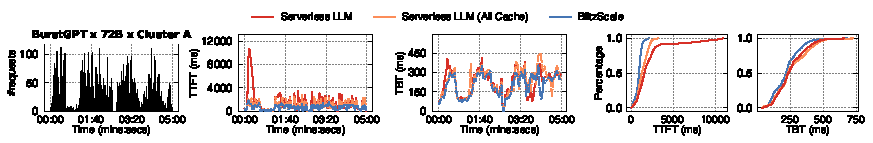
\includegraphics[width=1.01\textwidth,center]{./data/e2e-burstgpt.pdf} \\[0pt]
    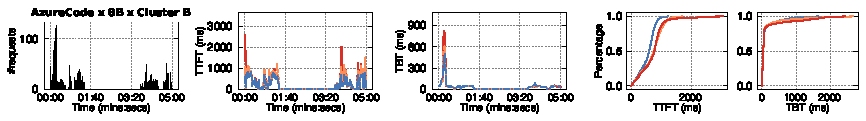
\includegraphics[width=1.01\textwidth,center]{./data/e2e-azurecode.pdf} \\[0pt]
    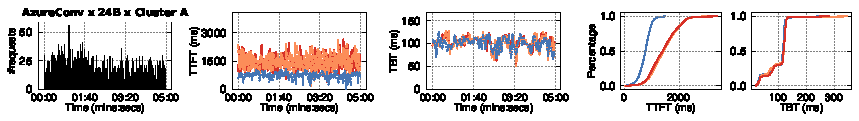
\includegraphics[width=1.01\textwidth,center]{./data/e2e-azureconv.pdf} \\[-5pt]
    \begin{minipage}{1\linewidth}
    \caption{\small{\textit{
        End-to-end performance comparison between {\sys} and {\base} on various workloads,
        models and clusters. 
    }}}
    \label{fig:eval-e2e}
    \end{minipage} \\[-10pt]
\end{figure*} 


\noindent
Due to space limitations,
for each model, we choose one trace on one of the clusters to evaluate the performance.
{\fig{fig:eval-e2e}} presents the end-to-end performance
when serving with a prefill and decode disaggregation setup
where the instances for different phases are scaled independently.
The first column shows the request rate of the trace,
the second and third columns show the mean TTFT and TBT, respectively,
where each point is the average latency measured during a small time window (1s),
and the final two columns present the cumulative distribution function (CDF) of the TTFT and TBT
during the evaluation period, respectively.
We focus on comparing with S-LLM and AllCache in this section
and leave the comparison with DistServe in the next section,
as it does not support autoscaling.

\stitle{Overall performance. }
First, we can see that {\sys} has the lowest TTFT and TBT in all workloads
thanks to the fast autoscaling speed.
Specifically,
on BurstGPT, the TTFT is 75.5\,\% and 21.1\,\% shorter than S-LLM and AllCache,
respectively,
and the TBT is 7.4\,\% and 5.1\,\% shorter, respectively.
Nevertheless,
the degrees of improvement are different across metrics
due to the unique characteristics of the prefill and decode phases.
Meanwhile,
the behaviors of systems, especially S-LLM, are different across workloads
due to the different request arrival patterns (see the first column).
We elaborate on the differences in the following.

\stitle{TTFT vs. TBT. }
{\sys} is more effective in reducing the TTFT than TBT on all workloads.
This is due to two reasons.
First, the decode instance can be pre-scaled 
thanks to our optimized policy (\textsection{\ref{sec:design-llm}}),
which we apply to all baselines. 
Specifically, 
when the prefill throughput increases,
{\sys} (and its baselines) will simultaneously scale the decode instances,
yet no more decode instances are needed at the scale time.
Thus, the scaling time is overlapped with the prefill time, 
which hides some scaling overheads.
Second,
decode scales less than prefill because
as long as there is sufficient memory on the decode instances,
all systems can handle decoding with a slightly increased TBT due to no queueing.
Since all models adopt modern LLM optimization group query attention~\cite{gqa}
with low memory footprint,
decoding instances are more sufficient than prefill instances.
Nevertheless, {\sys} still achieves a 5.1--7.4\,\%, 88.3--94.1\,\% and 0.7--1.8\,\%
shorter TBT than S-LLM and AllCache on three workloads, respectively.

\stitle{Comparisons between different workloads results. }
{\sys} always outperforms AllCache thanks to fast network-based autoscaling
as well as live scaling,
but S-LLM has different behaviors compared to AllCache in these workloads.
On BurstGPT, S-LLM first has a sharp TTFT spike at the first burst (time 0:05),
while it is close to AllCache in future bursts,
because future bursts can benefit from host cache.
In comparison, on AzureCode,
S-LLM has spikes under both bursts (time 0:05 and time 03:25),
because the gap between two bursts makes the host cache evicted due to a time-to-live policy.
Finally, on AzureConv,
since the bursts continuously arrive, S-LLM always hits the host cache,
so the performance---see the CDF graphs---is similar to AllCache.

\iffalse
First, {\sys} has 86.1\,\%, 55.5\,\%, 31.0\,\% shorter TTFT, 
and has 18.1\,\%, 57.8\,\% and 1.1\,\% shorter TBT than S-LLM, respectively. 
The reduction mainly comes from the fast autoscaling provided by 
our network-based scaling.
The penalties are obvious in 70\,B model: 
because loading its parameters from SSD is too slow. 
As shown in Table~\ref{tab:cluster}, our cluster only supports a 10\,Gbps per-GPU bandwidth,
so a 4-GPU 70\,B instance needs 28 seconds to load the parameters. 
Note that while all prefill workloads are affected by short bursts in the traces,
decode is relatively resilient.
This is because each decode will stay for a relative (unpredictable) long time, 
so the bursts are amortized (e.g., in AzureConv, decode instances seldom scale up or down). 
An exception is the AzureCode, where the decode also fluctuates with the prefill,
because its decode is much shorter than the others (with an average generated tokens of 28, which is 211 of AzureConv).

Second, {\sys} has close to AllCache performance in all workloads. 
This is because the network we used has a 78\,\% bandwidth of the host-GPU link,
and our live autoscaling can fill the missing gap by allowing the new instances to serve 
even with partial parameters loaded. 
An interesting phenomenon is that on AzureCode, 
we are even faster than AllCache,
because our LLM-trick can lively mutate a prefill instance to a decode instance, 
avoiding network traffic and thus realizing a zero-cost autoscaling. 
\fi

\subsection{Performance and resource usage}
\label{sec:eval-resource}

\begin{figure*}[!t]
    %\hspace{-3mm}
    \centering
    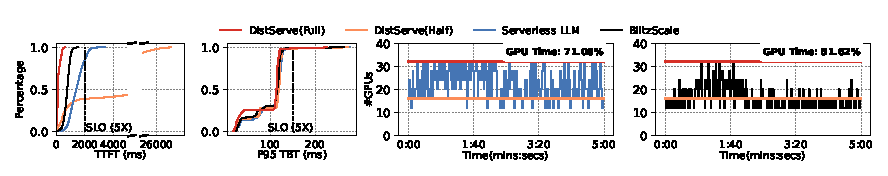
\includegraphics[width=1.01\textwidth,center]{./data/e2e-comparision-utilization-new.pdf}  \\[-10pt]
    \begin{minipage}{1\linewidth}
    \caption{\small{\textit{        
        A comparison between GPU usage under AzureConv with Mistral\,24B.
    }}}
    \label{fig:eval-e2e-gpu}
    \end{minipage} \\[-15pt]
\end{figure*} 

\nospacestitle{Comparison with non-autoscaling systems. }
We first compare {\sys} with DistServe. 
Since DistServe does not support autoscaling,
its performance is highly dependent on the number of provisioned instances.
Therefore, we evaluate two setups:
DistServe (full) uses all GPUs in our cluster and represents
an optimal performance at the cost of GPU waste.
On the other hand, DistServe (half) uses GPUs with the average number of instances
required to handle all the workloads within the evaluation period.
For simplicity, we only present the results on AzureConv on 24B models,
the overall trends are similar.
We have carefully calibrated DistServe's performance,
such that when autoscaling is disabled in {\sys},
DistServe has the same performance as {\sys} in all setups.


The first two columns of {\fig{fig:eval-e2e-gpu}} present the latency results. 
First, it can be observed that DistServe (full) has the best performance,
because the GPU is over-provisioned 
so it doesn't suffer from queueing or scaling overhead.
Nevertheless, {\sys} still achieves the same service level objective (SLO) as DistServe (full)
while S-LLM incurs 18.7\,\% SLO violations.
We follow the traditional 5\,$\times$ SLO~\cite{DBLP:conf/osdi/ZhongLCHZL0024}
since all our workloads (chat and code generation) are latency-sensitive.
Specifically, if a request's end-to-end (TTFT or TBT) latency is exceeds 5\,$\times$ the average latency,
it violates the SLO.
Finally, DistServe (half) has the poorest performance:
on average, {\sys} has a 95.8\,\% and 1\,\% shorter TTFT and TBT than DistServe (half).
{\sys} achieves this by using the same GPU time for serving this model as DistServe (half),
and this time is 50\,\% smaller than DistServe (full),
which we elaborate next.

\stitle{GPU time used. \,}
The last two columns of {\fig{fig:eval-e2e-gpu}} show the GPU time used by S-LLM
and {\sys}, respectively.
For S-LLM and {\sys},
we collected the aggregated GPU usage at each time point for both prefill and decode instances,
and the overall time is calculated by integrating the area under the curve.
For variants of DistServe, their GPU time is constant across the evaluation period.
We can see that {\sys} has 19.46\,\,\% lower GPU time than S-LLM
thanks to the fast autoscaling capability:
with low scaling speed,
there would be more queued requests, so the system would trigger more scaling operations
that use more GPU time.
This is unnecessary with {\sys}.
Even with less GPU time used,
{\sys} has a 48.1\,\% and 1.8\,\% shorter TTFT and TBT than S-LLM, respectively.

\begin{figure}[!t]
    %\hspace{-3mm}
    \centering
    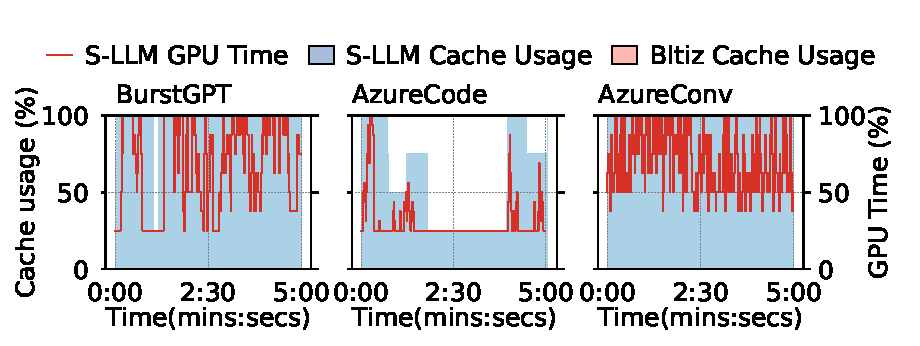
\includegraphics[width=1.0\linewidth,center]{./data/motiv-cache-usage-new.pdf}  \\[2pt]
    \begin{minipage}{1\linewidth}
    \caption{\small{\textit{        
        A comparison of host cache usage on S-LLM and {\sys} under the evaluated workloads.
    }}}
    \label{fig:eval-cache-usage}
    \end{minipage} \\[-20pt]
\end{figure} 

\stitle{Host cache usage. \,}
Compared to ServerlessLLM, {\sys}
also consumes less host memory for parameter caching. 
{\fig{fig:eval-cache-usage}} reports the host memory usage for different systems.
We omit AllCache and DistServe,
as AllCache always fully replicates parameters to all hosts while
DistServe does not need caching.
We normalize the host cache usage as different workloads use different clusters.
The results deliver two messages.
First, {\sys} only needs minimal host caching (less than one) to achieve fast autoscaling:
this is as expected by our design because
we prefer to load parameters from GPUs of instances that serve the model,
and even when no serving instance is available,
we only need one host copy due to the network-based multicast.
Second, the memory usage of ServerlessLLM is proportional to the number of hosts involved in the serving,
so a model can quickly ``pollute'' the host cache.
This is non-optimal for an {\maas} system because it can simultaneously
serve many models while the host cache is limited.

\iffalse
we use logical hosts to simulate a larger evaluation setup. 
Specifically, 
for 70\,B workloads, we logically group 4-GPU to a host, which allows us to 
simulate the performance with 16 hosts.
For 7\,B and 8\,B workloads, we use 1-GPU for each host,
allowing us to simulate a larger cluster with 32 and 16 hosts, respectively.
Note single-GPU hosts are common in serving clusters~\cite{DBLP:conf/osdi/SunHZXZL024}. 

We measure the cache as follows. For {\sys},
we only maintain at least one copy of the model across all the hosts,
so its cache usage is always 1. 
For S-LLM, we follows its default setting, which uses a 5-minute time-to-live time.
The model is cached on the host for 5 minutes after the last request.
As we can see, {\sys} has orders of magnitude smaller host cache usage.
Such a reduction can free more memory for other models, which can subsequently improve their performance. 
On BurstGPT, S-LLM has a slightly better overall cache usage, 
because there are many time in BurstGPT with no requests, 
which means that S-LLM will not cache any model on the host due to the time-to-live policy.
Nevertheless, as we have extensively shown such a cache miss will cause a significant performance penalty
during auto scale. 
\fi

\subsection{Detailed performance analysis}
\label{sec:eval-ablation}

\begin{figure*}[!t]
    %\hspace{-3mm}
    \centering
    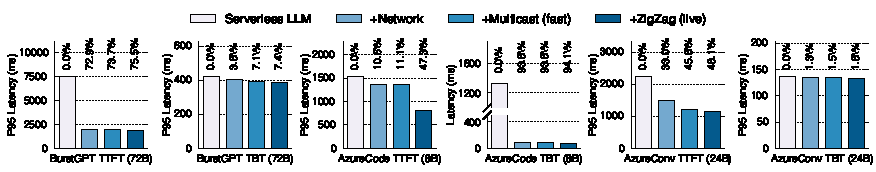
\includegraphics[width=1.01\textwidth,center]{./data/abl-new.pdf}  \\[-2pt]
    \begin{minipage}{1\linewidth}
    \caption{\small{\textit{        
        An ablation study on the effectiveness of our proposed techniques. 
    }}}
    \label{fig:eval-alb}
    \end{minipage} \\[-20pt]
\end{figure*} 

\begin{figure}[!t]
    %\hspace{-3mm}
    \centering
    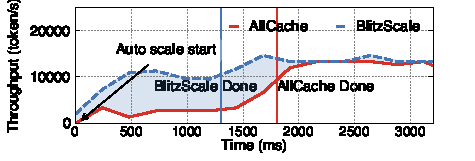
\includegraphics[width=1.0\linewidth,center]{./data/ext.pdf}  \\[2pt]
    \begin{minipage}{1\linewidth}
    \caption{\small{\textit{        
    A detailed look at how {\sys} and AllCache scale a 24\,B model to 
    6 prefill instances on cluster A.
    }}}
    \label{fig:scale-breakdown}
    \end{minipage} \\[-5pt]
\end{figure} 

\nospacestitle{A detailed look at the live scale. }
{\fig{fig:scale-breakdown}} shows a throughput timeline
when using {\sys} and AllCache to scale six 24\,B prefill instances.
{\sys} utilizes two broadcast chains (each involving 3 instances),
while the end instances involve a live autoscale. 
The start instances are the decode instances.
For AllCache, it directly loads the parameters from the host memory of the scaled instances.
We can see that first, even with a few loaded layers (e.g., at time 500\,ms),
{\sys} can gradually emit tokens as a result of live execution.
Second, {\sys} can scale faster even compared with AllCache,
thanks to our NVLink-based fused link transmission protocol:
it can finish scaling in 1,200\,ms while AllCache takes about 2,000\,ms.


\stitle{Ablation study. }
{\fig{fig:eval-alb}} conducts an ablation study on the effectiveness of our proposed techniques.
We measured the effectiveness by incrementally enabling different techniques and reporting
the results on the three workloads:
``+Network'' leverages fast computing network instead of SSD for autoscaling,
``+Multicast (fast)'' further applies our optimized parameter broadcast protocol described in \textsection{\ref{sec:design-plan}},
while ``+ZigZag (live)'' enables live autoscaling of \textsection{\ref{sec:design-pp}}.

First, we can see that all techniques are effective in improving the end-to-end serving performance,
but the degrees differ across workloads.
First, ``+Network'' improves the scaling performance in all workloads thanks to the
higher bandwidth for the autoscaling data plane.
Second, ``+Multicast (fast)'' is effective in AzureCode and AzureConv,
but it is less effective in BurstGPT
due to the limitations of our cluster (up to 8 instances can be scaled
on 72\,B model),
so there are no cases to simultaneously scale multiple instances,
which is the targeted case for this technique.
Live autoscaling is mostly effective in AzureCode because it is evaluated on a cluster with
slow networking (Cluster B).
Finally, our techniques are not such effective on decoding because decode instances are sufficient in most cases,
which we have discussed in \textsection{\ref{sec:eval-app}}.
One exception is AzureCode:
in this workload, 
the prefill throughput increases slower than others (see the first column of {\fig{fig:eval-e2e}}),
so the decode instances are triggered later.
As a result, 
the slow scale of ServerlessLLM's SSD cannot be hidden,
making a faster scaling more beneficial.

\iffalse
We conclude our study of efficient autoscaling with an ablation study
on the effectiveness of our proposed techniques.
{\fig{fig:eval-alb}} presents the results on all the three workloads. 
We 
First, we can see that using network multicast for scaling (+Network) 
can significantly improve the autoscaling performance, which in turn 
improves the average TTFT and TBT. 
There is a outlier, the TBT in AzureConv. 
This is because the decode workloads is relative stable on it so it nearly meets no 
scaling during our evaluation. 
The improvement is most obvious in BurstGPT where we evaluated with a 70\,B model,
because SSD is far from achieving an efficient autoscaling (discussed in details in \textsection{\ref{sec:eval-app}}).
Second, an interference scale plan reduces the TTFT and TBT 
across various workloads by 0.4--5\,\%. 
The improvement is marginal because even without the plan, 
we still have a chance to scale the instance without interference.
Finally, live autoscaling further reduces the latencies by up to 40\,\% on AzureCode TBT. 
This makes {\sys} even faster than AllCache.
This is because AzureCode requires scaling multiple decode instances while its prefill instances 
are relatively spare.
Thus, we can directly mutate a prefill instance to a decode instance while lively scaling another prefill instance 
for remedy. 
\fi

\begin{figure}[!t]
    %\hspace{-3mm}
    \centering
    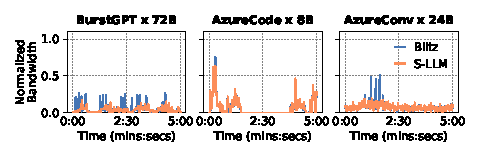
\includegraphics[width=1.0\linewidth,center]{./data/network-util.pdf}  \\[-10pt]
    \begin{minipage}{1\linewidth}
    \caption{\small{\textit{        
        A profile of the network usage of {\sys} (Blitz). 
    }}}
    \label{ffig:eval-network-util}
    \end{minipage} \\[-10pt]
\end{figure}


\stitle{Network usage. }
{\fig{ffig:eval-network-util}} shows the network usage of {\sys} and S-LLM:
we can see that though {\sys} leverages compute network for autoscaling 
and the scale frequency is high (see the last column of {\fig{fig:eval-e2e-gpu}}),
the additional network usage is negligible.

\begin{figure}[!t]
    %\hspace{-3mm}
    \centering
    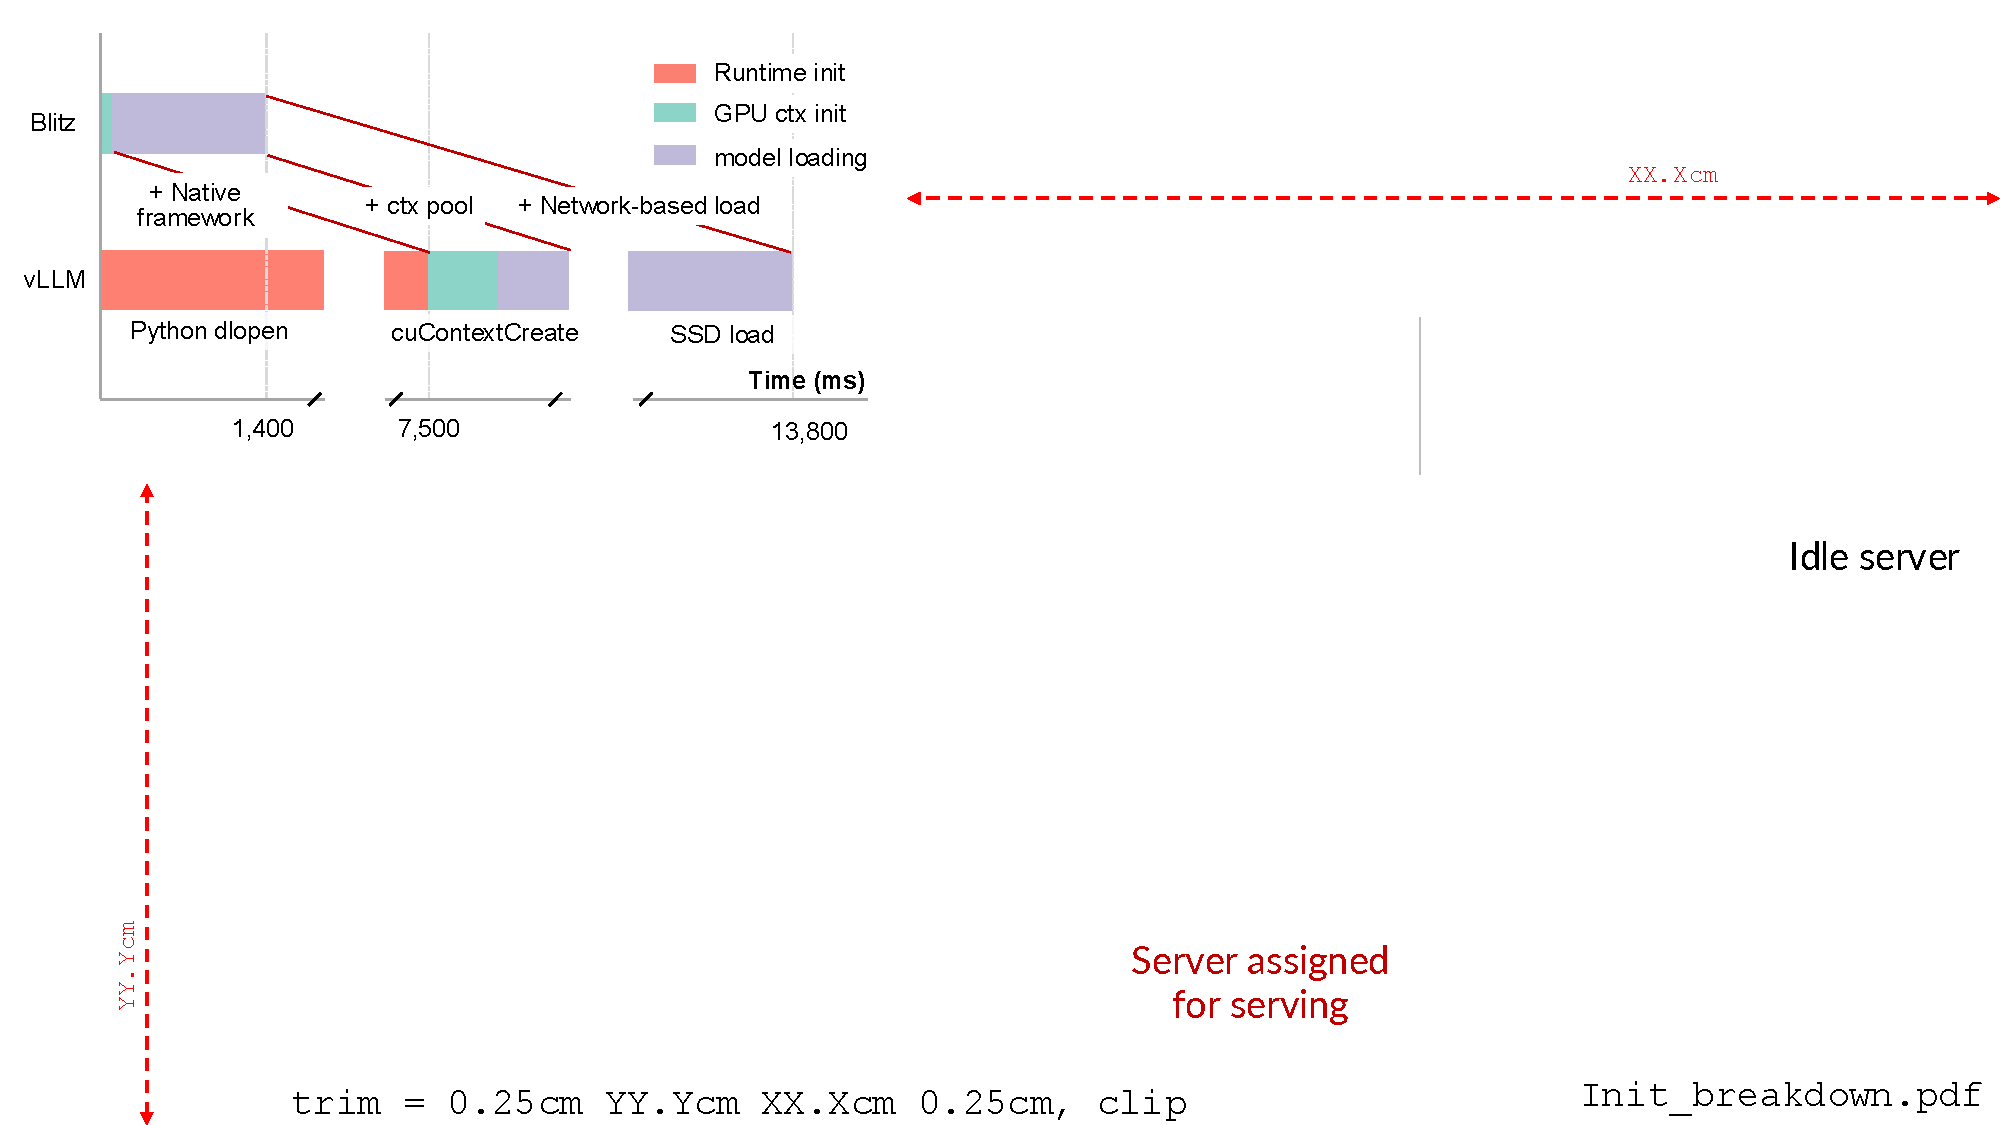
\includegraphics[width=.95\columnwidth, trim=0.25cm 10.9cm 18.55cm 0.9cm, clip]{figs/init_breakdown.pdf}  
    \\[-8pt]
    \begin{minipage}{1\linewidth}
    \caption{\small{\textit{        
        A comparison of init time of {\sys} and vLLM
    }}}
    \label{fig:breakdown}
    \end{minipage} \\[-10pt]
\end{figure}


\stitle{Control plane vs. data plane of model autoscaling. }
{\fig{fig:breakdown}} compares the control plane and data plane overhead during model autoscaling
with vLLM. 
We can see that with proper optimizations,
the control plane overhead is negligible.

\subsection{Performance under LLM PD colocation}
\label{sec:eval-pd-colocation}

\begin{figure}[!t]
    %\hspace{-3mm}
    \centering
    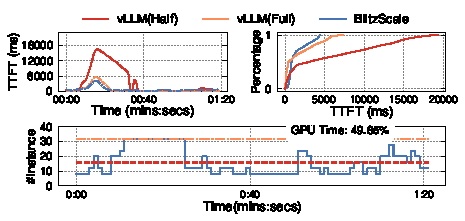
\includegraphics[width=1.0\linewidth,center]{./data/e2e-collocation-burstgpt.pdf}  \\[2pt]
    \begin{minipage}{1\linewidth}
    \caption{\small{\textit{        
        A comparison of {\sys} and vLLM on the BurstGPT workload. 
    }}}
    \label{fig:eval-colocation}
    \end{minipage} \\[-10pt]
\end{figure}



% \begin{minipage}{1\linewidth}
%     \hspace{-1mm}
%     \centering    
%     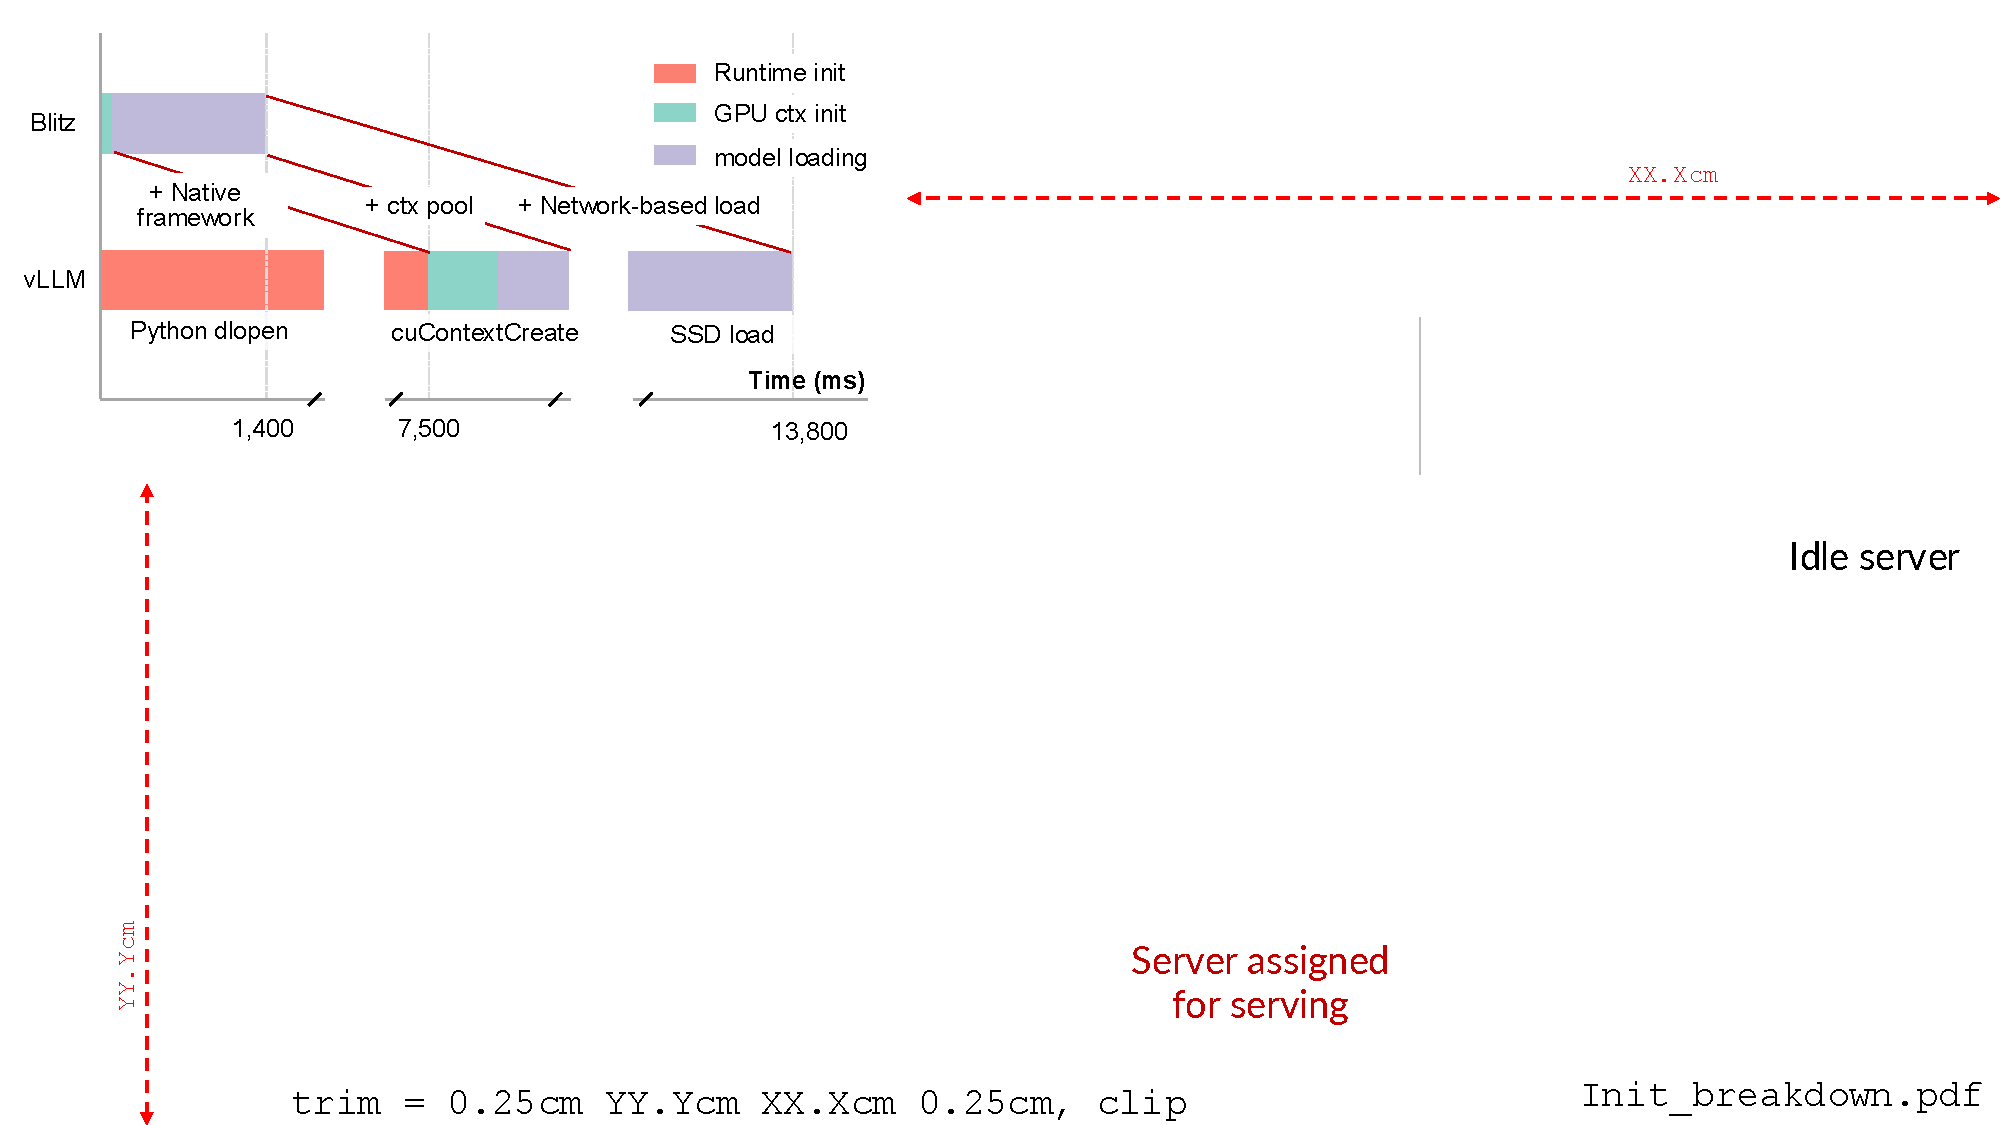
\includegraphics[width=.95\columnwidth, trim=0.25cm 8.83cm 17.27cm 0.25cm, clip]{figs/init_breakdown.pdf} 
%     \end{minipage} \\[8pt]
%     \begin{minipage}{1\linewidth}
%     \caption{\small{\textit{
%         A comparision of init time of {\sys} and vLLM
%     }}}
%     \label{fig:breakdown}
%     \end{minipage} \\[-10pt]
%     \end{figure*} 

\noindent
Finally, {\fig{fig:eval-colocation}} compares the performance of {\sys} and vLLM
where the serving is conducted in PD colocation on BurstGPT workloads with Llama2-7B model.
The general trend is similar to PD disaggregation:
{\sys} has comparable performance with over-provisioned vLLM,
while compared with an average provisioning,
{\sys} has a 0.24\,$\times$ shorter P99 TTFT.
Interestingly, we found {\sys} has even shorter tail TTFT compared with over-provisioned vLLM,
because our scheduling framework is optimized for cluster serving.